\section{Experiments}
\label{sec:exp}\label{sec:experiments}

All numbers are errors on real frames of the downstream model after 150 epochs (50 where noted); depth MSE in $\mathrm{mm}^2$, contact MAE in mm, normals and rotation in degrees. Sections~\ref{sec:kshot}--\ref{sec:qual} evaluate MAPL; Sections~\ref{sec:loo}--\ref{sec:fidelity} report the leakage-controlled renderer study that provides its baselines.


\begin{figure*}[t]
    \centering
    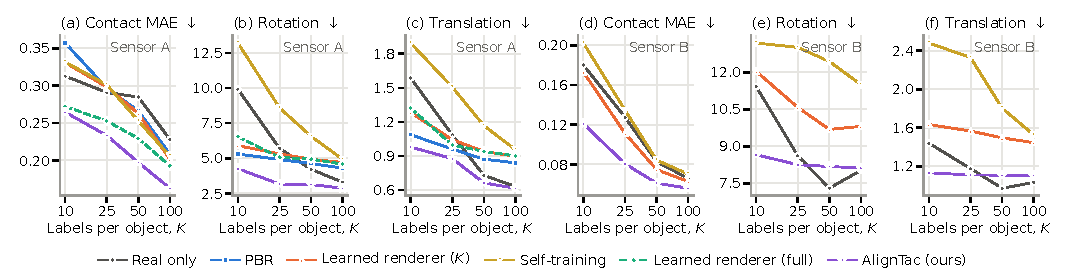
\includegraphics[width=0.95\textwidth]{figures/fig_kshot.pdf}
    \caption{\textbf{Label efficiency} (real validation error vs.\ labeled frames per object). The leakage-free learned renderer separates from real-only training only at $\Kreal=50$ and the physical renderer never improves dense error, while the leaky renderer (dashed) appears to help everywhere. MAPL improves dense error at every budget and passes the leaky renderer at $\Kreal=100$.}
    \label{fig:kshot}
\end{figure*}

\begin{table}[!tbp]
\centering
\tableformat
\caption{\textbf{$\Kreal$-shot with a shared real budget.} Every object contributes $\Kreal$ real frames; GAN-$\Kreal$ is trained on the same frames. MAPL and self-trained rows additionally use the unlabeled training frames (Sec.~\ref{sec:unlabeled}); refiner rows use no label at all. Real validation split ($472$ frames). Leaky rows use the renderer trained on all real pairs (the $\Kreal=10$ leaky row is a 50-epoch run).}
\label{tab:kshot}
\begin{tabularx}{\columnwidth}{lXrrrrr}
\toprule
$\Kreal$ & Training data & \metrichead{Depth}{MSE} & \metrichead{Contact}{MAE} & \shortstack[c]{\strut IoU\\\strut $\uparrow$} & \metrichead{Normal}{(deg)} & \metrichead{Rot.}{(deg)} \\
\midrule
\tabkshot
\bottomrule
\end{tabularx}
\end{table}

\subsection{Label Efficiency}
\label{sec:kshot}
Table~\ref{tab:kshot} and Fig.~\ref{fig:kshot} compare, at equal label budget, real-only training, co-training with either renderer, self-training on the teacher's own predictions (Sec.~\ref{sec:ablation}) and MAPL. Each MAPL run uses the $2{,}997$--$4{,}077$ training frames outside the $\Kreal$ budget without their labels.

\noindent\textbf{Simulation alone.} Neither leakage-free renderer improves dense error for $\Kreal\le25$; the learned renderer helps from $\Kreal=50$ (depth MSE $-10\%$, $-16\%$ at $\Kreal=100$), the physical renderer by at most $5\%$. Both lower rotation error at $\Kreal=10$ ($9.6^\circ\!\to\!5$--$6^\circ$) and raise it at $\Kreal=100$.

\noindent\textbf{MAPL} improves on real-only training at every budget: depth MSE by $13\%$, $19\%$, $36\%$ and $37\%$ and contact MAE by $13\%$, $20\%$, $27\%$ and $28\%$ at $\Kreal=10$, $25$, $50$ and $100$, with IoU $+0.06$ to $+0.08$ and normal error $-2.6^\circ$ to $-5.1^\circ$. Over three seeds (50 epochs) the depth MSE is $0.0558\pm0.0003$, $0.0447\pm0.0009$, $0.0313\pm0.0007$ and $0.0229\pm0.0003$ against $0.0635\pm0.0007$, $0.0551\pm0.0010$, $0.0480\pm0.0006$ and $0.0366\pm0.0008$ for real-only training. Three comparisons put the gain in perspective. MAPL with $50$ labels per object ($0.0307$) is ahead of real-only training with $100$ ($0.0369$) and on par with the learned renderer at $100$ ($0.0311$). At $\Kreal=100$ it is \emph{better} than the leaky renderer (depth MSE $0.0232$ vs.\ $0.0274$, contact MAE $0.168$ vs.\ $0.205$), and at $\Kreal=25$ it matches the leaky contact MAE and IoU at $8\%$ higher depth MSE. Its rotation error is the lowest leakage-free value for $\Kreal\le50$ ($4.0^\circ$, $3.7^\circ$, $3.7^\circ$); at $\Kreal=100$ real-only training is ahead ($3.2^\circ$ vs.\ $3.7^\circ$) until the aligner is also used at test time (Sec.~\ref{sec:tta}). MAPL does not need the renderer for these numbers: with a real-only teacher, an aligner trained on the $\Kreal$ frames alone and no synthetic frame at all (``no renderer''), depth MSE is $0.0521$, $0.0433$, $0.0291$ and $0.0227$ and rotation error $2.5$--$4.7^\circ$, equal to or better than with the renderer; the renderer earns its place across sessions (Sec.~\ref{sec:cross}).

\begin{table}[!tbp]
\centering
\tableformat
\caption{\textbf{Seeds.} Mean $\pm$ standard deviation over three seeds (50 epochs) on the real validation split. ``+ MAPL'': real-only teacher, no synthetic frame; ``with renderer'': the configuration of Table~\ref{tab:kshot}.}
\label{tab:seeds}
\setlength{\tabcolsep}{2.0pt}
\footnotesize
\begin{tabularx}{\columnwidth}{@{}rXcccc@{}}
\toprule
$\Kreal$ & Training data & Depth MSE & Cont.\ MAE & IoU & Rot. \\
\midrule
\tabseeds
\bottomrule
\end{tabularx}
\end{table}

\noindent\textbf{Seeds.} Table~\ref{tab:seeds} repeats the main comparison with three seeds: the standard deviations are an order of magnitude below the differences between methods.

\begin{table}[!tbp]
\centering
\tableformat
\caption{\textbf{Alignment ablation} ($\Kreal=25$, 50 epochs; first, fifth and last row are three-seed means). Left: quality of the pseudo labels of the unlabeled frames against their withheld true labels (evaluation only). Right: real validation error of the model trained on them. Depth label: teacher prediction or mesh depth at the fitted pose ($^{1/2}$: mesh on the half of each object's frames with the lowest render error, teacher on the rest). Pose label: none (pose loss on the $\Kreal$ labeled frames only), teacher pose, pose found by L1 render-and-compare search with GAN-$\Kreal$ ($^{1/2}$: on the confident half only), or the learned aligner. $\ddagger$: synthetic data from the teacher-pair renderer; $\dagger$: MAPL (renderer retrained on the aligned pairs).}
\label{tab:rcabl}
\setlength{\tabcolsep}{3pt}
\resizebox{\columnwidth}{!}{%
\begin{tabular}{@{}llrrrrrrr@{}}
\toprule
\multicolumn{2}{c}{Labels of $U$} & \multicolumn{3}{c}{Pseudo-label quality} & \multicolumn{4}{c}{Downstream} \\
\cmidrule(lr){1-2}\cmidrule(lr){3-5}\cmidrule(lr){6-9}
Depth & Pose & \shortstack[c]{\strut IoU\\\strut $\uparrow$} & \metrichead{Cont.}{MAE} & \metrichead{Rot.}{(deg)} & \metrichead{Depth}{MSE} & \metrichead{Cont.}{MAE} & \shortstack[c]{\strut IoU\\\strut $\uparrow$} & \metrichead{Rot.}{(deg)} \\
\midrule
\tabrcabl
\bottomrule
\end{tabular}}
\end{table}

\begin{figure}[!tbp]
    \centering
    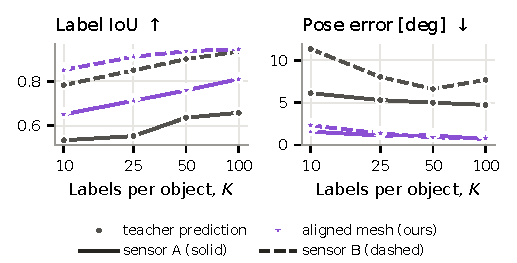
\includegraphics[width=\columnwidth]{figures/fig_labels.pdf}
    \caption{\textbf{Label quality on the unlabeled frames} against their withheld reference labels (evaluation only): the $\Kreal$-shot teacher's own prediction versus the mesh at the aligned pose. The aligner improves on the teacher at every budget on both sensors.}
    \label{fig:labels}
\end{figure}

\subsection{Why Alignment: Ablation}
\label{sec:ablation}\label{sec:unlabeled}
Table~\ref{tab:rcabl} varies only how the unlabeled frames are labeled.

\noindent\textbf{Self-training.} With the teacher's own depth as label (stitched from five windows to cover the full frame, pose loss on the labeled frames only), depth MSE improves by $8\%$ but contact MAE and IoU do not: the pseudo labels inherit the teacher's localization error (label IoU $0.56$), so the student learns sharper depth values, not where the contact is. Adding the teacher's pose as a label restores rotation accuracy and nothing else, and a second round of self-training changes depth MSE by at most $4\%$ in either direction.

\noindent\textbf{L1 render-and-compare.} Replacing the aligner by a search---fit the mesh to the teacher depth on a pose grid, then pick, among $567$ neighbouring poses, the one whose GAN-$\Kreal$ render is closest to the frame in image L1---helps less (label IoU $0.64$, pose error $2.5^\circ$) and requires gating: on the half of the frames with the larger render error the mesh label is no better than the teacher's. The few-shot renderer is a poor comparator; at $\Kreal=25$ its render at the true pose is farther from the frame than its render at the selected pose on $93\%$ of the frames.

\noindent\textbf{Learned aligner.} The aligner lowers the teacher's pose error from $5.3^\circ$ to $1.1^\circ$ on the $3{,}897$ unlabeled frames and yields labels with IoU $0.71$ and contact MAE $0.24\,$mm (teacher: $0.55$, $0.32$). Label quality grows with the budget (IoU $0.65$, $0.71$, $0.76$, $0.81$ and pose error $1.6^\circ$, $1.1^\circ$, $1.1^\circ$, $0.7^\circ$ for $\Kreal=10$--$100$). The student trained on these labels is the first to lower contact error ($0.310\!\to\!0.246$) and to raise IoU ($0.624\!\to\!0.729$). Further findings: (i) the aligner is learned from the $\Kreal$ real frames---adding frames rendered by GAN-$\Kreal$ at random poses does not change label quality (IoU $0.72$), and training on such renders alone fails ($0.56$); (ii) no gate is needed, since on the frames a render-error gate would reject its labels still beat the teacher's (IoU $0.66$ vs.\ $0.55$); (iii) it is insensitive to its settings (half or double the perturbation range: $0.72$, $0.73$; 2k or 20k steps: $0.73$, $0.72$; ResNet-34 or -50 backbone: $0.73$, $0.71$), while dropping the ImageNet initialization costs accuracy ($0.67$); (iv) the student is unchanged whether its synthetic frames come from the renderer retrained on aligned pairs or on teacher-labeled pairs (depth MSE $0.0447$ in both cases), and within the session it does not need them at all (last row: $0.0433\pm0.0004$ over three seeds with a real-only teacher and no synthetic frame, against $0.0447\pm0.0009$ with the renderer); (v) a quarter of the unlabeled frames already gives most of the gain (depth MSE $0.0453$, $0.0452$ and $0.0447$ with $25\%$, $50\%$ and $100\%$ of $U$), while IoU keeps growing with their number ($0.710$, $0.725$, $0.729$); (vi) a second round, with the student as the new teacher, does not improve further: although the student proposes poses $1.5^\circ$ closer than the original teacher, the aligned labels (IoU $0.65$, $0.71$ at $\Kreal=10$, $25$) and the retrained student (depth MSE $0.0570$, $0.0445$; IoU $0.674$, $0.717$) are within seed variation of the first round. An unpaired sim-to-real refiner of the physical render, which uses the unlabeled frames without any pose, does not improve on its input (contact MAE $0.349$ vs.\ $0.346$ on unseen objects).

\noindent\textbf{Self-trained renderer.} Following self-training~\cite{lee2013pseudo,xie2020noisy}, the $\Kreal$-shot downstream model pseudo-labels $U$ (depth predicted on five windows and stitched back to the full frame; frames kept when the predicted contact overlaps the image's black-hat ridge mask, IoU $\ge0.2$: $3{,}260$ frames at $\Kreal=25$, $2{,}677$ at $\Kreal=100$), and GAN-$\Kreal$ is retrained on the $\Kreal$ true plus the pseudo pairs. The pseudo labels are as accurate as the labeler ($0.32$ and $0.24\,$mm contact MAE against the withheld true labels), and the renderer's fidelity improves by $5\%$ at both budgets ($0.108\!\to\!0.102$, $0.077\!\to\!0.073$), which the proxy translates into a $1\%$ downstream gain: depth MSE $0.0544\!\to\!0.0538$ at $\Kreal=25$ and $0.0311\!\to\!0.0308$ at $\Kreal=100$ (contact MAE $0.207$, the best leakage-free value at $\Kreal=100$). With teacher labels the renderer thus gains little from more real images. With the aligned pairs of step~2 it gains more: contact-region error falls by $13$--$19\%$ at every budget ($0.121\!\to\!0.105$ at $\Kreal=10$, $0.108\!\to\!0.090$ at 25, $0.095\!\to\!0.077$ at 50, $0.077\!\to\!0.065$ at 100; leaky $0.057$), the best strict renderers of the study, although swapping this renderer for the teacher-pair one leaves the downstream error of the aligned model unchanged (Table~\ref{tab:rcabl}): once the real frames carry good labels, the synthetic frames matter little.

\noindent\textbf{Window stitching.} Without alignment the label is the teacher depth, and labeling $U$ on the center window alone leaves the pseudo depth empty outside the $0.816$ crop (pseudo-label contact MAE $0.41\,$mm over the full frame instead of $0.32$). The self-trained model then has the same depth MSE ($0.0518$ vs.\ $0.0517$, model only, $\Kreal=25$; Table~\ref{tab:kshot}) but a worse contact MAE ($0.328$ vs.\ $0.300$) and a $30\%$ larger peak-depth error, and the gap persists across sessions (contact MAE $0.358$ vs.\ $0.318$): the rotation augmentation brings the frame border into the training crop, where unstitched labels are wrong.

\noindent\textbf{Rounds.} Without alignment, relabeling $U$ with $f_1$ and repeating the renderer and model steps improves the pseudo labels at $\Kreal=25$ (label IoU $0.56\!\to\!0.60$, contact MAE $0.32\!\to\!0.31\,$mm, $3{,}516$ frames kept instead of $3{,}260$) but not at $\Kreal=100$ ($0.66\!\to\!0.65$), and the downstream change is small in both directions: depth MSE $0.0508\!\to\!0.0500$ and IoU $0.628\!\to\!0.642$ at $\Kreal=25$, $0.0285\!\to\!0.0295$ and $0.750\!\to\!0.736$ at $\Kreal=100$, rotation unchanged ($6.2^\circ$, $4.9^\circ$). The labeler's localization error is not something its own student can correct; the alignment step is. With alignment a second round changes nothing either (item (vi) above): one round of MAPL saturates.

\begin{table}[!tbp]
\centering
\tableformat
\caption{\textbf{Cross-session.} Sensor-A models evaluated on the curated session-2 set ($854$ frames, 11 objects; poses re-estimated per frame and manually reviewed). Rot.: raw; Rot.$^{\ast}$: after removing a per-object constant offset (the re-placement of the object). All models use the full session-1 real set unless a $\Kreal$ is given.}
\label{tab:cross}
\begin{tabularx}{\columnwidth}{Xrrrrr}
\toprule
Training data & \metrichead{Contact}{MAE} & \shortstack[c]{\strut IoU\\\strut $\uparrow$} & \metrichead{Normal}{(deg)} & \metrichead{Rot.}{(deg)} & \metrichead{Rot.$^{\ast}$}{(deg)} \\
\midrule
\tabcross
\bottomrule
\end{tabularx}
\end{table}

\subsection{A Second Session}
\label{sec:cross}
On the second session (Table~\ref{tab:cross}) dense error is $1.5$--$3\times$ the same-session value, partly because the reference poses are re-estimated. The ordering of the methods is preserved. MAPL has the lowest contact MAE and the highest IoU of its budget ($0.310$, $0.660$ at $\Kreal=25$; $0.252$, $0.743$ at $\Kreal=100$), i.e.\ $16\%$ and $28\%$ less contact error than real-only training, as within the session; at $\Kreal=100$ it is ahead of the model trained on \emph{all} session-1 labels ($0.315$, $0.675$) and level with that model's leaky variant. Simulation also helps across sessions (contact MAE $0.315\!\to\!0.27$--$0.29$ and rotation $16.4^\circ\!\to\!10.5$--$11.5^\circ$ for the full-data model). Here the synthetic frames matter: without the renderer MAPL loses its advantage over self-training at $\Kreal=100$ (contact MAE $0.288$, IoU $0.707$), although it is as accurate within the session---the renderer's contribution is robustness to the appearance of a new session, consistent with Sec.~\ref{sec:study}. Raw rotation error remains above $10^\circ$ for every method because the objects were re-placed; two thirds of it is a per-object constant.

\noindent\textbf{Renderer baselines across sessions.} Table~\ref{tab:cross} evaluates the sensor-A models on the second capture. Dense error is $1.5$--$3\times$ the same-session value (e.g.\ contact MAE $0.315\,$mm against $0.117$ for the model trained on all session-1 real data), partly because the reference poses are re-estimated; the informative quantity is the ordering. Simulation helps every task across sessions. With the full session-1 real set, contact MAE falls from $0.315\,$mm (real only) to $0.29$ with the physical and $0.27$ with the learned renderer, IoU rises from $0.675$ to $0.69$--$0.70$ and $0.72$--$0.73$, normal error falls from $25.4^\circ$ to $24.0$--$24.9^\circ$ with the calibrated and learned renderers, and raw rotation error drops from $16.4^\circ$ to $9.7$--$11.5^\circ$; the geometry control ($28.7^\circ$) shows that the pose gain again comes from mesh coverage. The domain-randomized renderer matches the calibrated one on dense error ($0.294$, IoU $0.691$) and is slightly behind on pose ($12.3^\circ$), as on unseen objects: randomized appearance degrades the contact-silhouette signal. About $2/3$ of the remaining rotation error is a per-object constant (Rot.$^{\ast}$ $4.7$--$6.5^\circ$ for every model), i.e.\ the re-placement offset rather than a perception error. In the $\Kreal$-shot regime the dense gain grows with $\Kreal$: at $\Kreal=25$ only the learned renderer lowers contact MAE ($0.368\!\to\!0.342$), at $\Kreal=100$ both renderers do ($0.351\!\to\!0.295$--$0.299$) and the learned one also raises IoU ($0.657\!\to\!0.713$) and lowers rotation error ($17.5^\circ\!\to\!13.7^\circ$), whereas simulation-only training does not transfer dense geometry across sessions (IoU $0.56$, normal $51^\circ$): the session-invariant part of the synthetic data is its geometry, not its appearance.

\begin{table}[!tbp]
\centering
\tableformat
\caption{\textbf{Test-time alignment.} Rotation error (deg) of the predicted pose and after six aligner iterations against the object mesh. No retraining.}
\label{tab:poseref}
\setlength{\tabcolsep}{3.5pt}
\begin{tabular}{@{}rrrrrrrrr@{}}
\toprule
& \multicolumn{4}{c}{Validation (session 1)} & \multicolumn{4}{c}{Session 2} \\
\cmidrule(lr){2-5}\cmidrule(lr){6-9}
& \multicolumn{2}{c}{Real only} & \multicolumn{2}{c}{MAPL} & \multicolumn{2}{c}{Real only} & \multicolumn{2}{c}{MAPL} \\
$\Kreal$ & pred. & +align & pred. & +align & pred. & +align & pred. & +align \\
\midrule
\tabposeref
\bottomrule
\end{tabular}
\end{table}

\subsection{Test-Time Alignment}
\label{sec:tta}
Since pose is defined with respect to a known object, the $\Kreal$-shot aligner can refine the pose predicted on a test frame (Table~\ref{tab:poseref}). On the validation split rotation error falls from $3.2$--$9.6^\circ$ to $0.4$--$2.8^\circ$ for real-only models and from $3.7$--$4.0^\circ$ to $0.8$--$1.5^\circ$ for MAPL models; from $\Kreal=25$ on the refined error is about $1^\circ$ whichever model proposes the pose, and translation error falls by $25$--$50\%$. On the second session rotation error falls from $13$--$20^\circ$ to $5$--$11^\circ$ (real only) and from $9$--$11^\circ$ to about $5^\circ$ (MAPL) with a median of $1.5$--$2.2^\circ$: the mean is dominated by a minority of frames on which the alignment fails. The mesh at the aligned pose is also a depth estimate: on the validation split it is as accurate as the MAPL student's output (IoU $0.81$ vs.\ $0.79$, contact MAE $0.158$ vs.\ $0.168\,$mm at $\Kreal=100$) and lifts a real-only model to the MAPL level (IoU $0.656\!\to\!0.710$ at $\Kreal=25$), so the student distills into a mesh-free network what alignment achieves with the mesh. The aligner also generalizes across objects: trained on the nine seen objects of the leave-object-out protocol and applied to the three held-out ones, whose only available data is their mesh, it lowers the rotation error of the simulation-trained models of Table~\ref{tab:loo} from $4.8$--$6.8^\circ$ to $0.6$--$1.0^\circ$.

\begin{table}[!tbp]
\centering
\tableformat
\caption{\textbf{Second sensor (\sensorB{}) with mesh-registered labels}; $1{,}620$ test frames, 50 epochs. ``no renderer'': real-only teacher and no synthetic frame. Self-training uses the teacher's own depth as label.}
\label{tab:sbmapl}
\setlength{\tabcolsep}{2.4pt}
\begin{tabularx}{\columnwidth}{@{}rXrrrrr@{}}
\toprule
$\Kreal$ & Training data & \metrichead{Depth}{MSE} & \metrichead{Contact}{MAE} & \shortstack[c]{\strut IoU\\\strut $\uparrow$} & \metrichead{Normal}{(deg)} & \metrichead{Rot.}{(deg)} \\
\midrule
\tabsbmapl
\bottomrule
\end{tabularx}
\end{table}

\subsection{A Second Sensor}
\label{sec:sensorb}
\noindent\textbf{MAPL.} On \sensorB{} ($1{,}620$ test frames) MAPL transfers without any change of settings (Table~\ref{tab:sbmapl}, Fig.~\ref{fig:kshot}d). The public depth labels of this dataset are not mesh projections, so we re-registered them: the mesh pose that best explains each label was fitted ($0.018\,$mm mean residual) and canonicalized against the object's rotational symmetry, and every method was retrained and tested on these mesh-registered labels. The few-shot teacher is already accurate on this sensor (label IoU $0.78$, $0.85$, $0.90$, $0.93$ on the unlabeled frames at $\Kreal=10$, $25$, $50$, $100$; $0.55$ at $\Kreal=25$ on sensor A), yet the aligner improves on it at every budget (IoU $0.85$, $0.91$, $0.94$, $0.95$; pose error $2.3^\circ$, $1.4^\circ$, $0.9^\circ$, $0.8^\circ$ against $6.6$--$11.4^\circ$). At $\Kreal=25$ the student lowers depth MSE from $0.0179\pm0.0004$ to $0.0075\pm0.0001$ and contact MAE from $0.127\pm0.001$ to $0.078\pm0.0003\,$mm over real-only training (three seeds) and raises IoU from $0.849$ to $0.903$. The baselines gain far less: the learned renderer trained on the $25$ pairs reaches $0.111\,$mm (IoU $0.877$) and self-training on the teacher's depth does not improve on real data ($0.135\,$mm, $0.846$). Without any synthetic frame, MAPL lowers contact MAE from $0.180$, $0.127$, $0.083$, $0.066$ to $0.121$, $0.081$, $0.061$, $0.056\,$mm at $\Kreal=10$--$100$ ($-15$ to $-36\%$) and depth MSE by $33$--$58\%$, so that, as on sensor A, it needs about half the labels of real-only training for a given contact error. Rotation error improves at $10$ and $25$ labels ($14.0^\circ\!\to\!9.5^\circ$, $13.4^\circ\!\to\!9.2^\circ$) but not beyond ($9^\circ$ either way). Scored against the original public labels, MAPL keeps its advantage (contact MAE $0.137\!\to\!0.098\,$mm at $\Kreal=25$).

\begin{table}[!tbp]
\centering
\tableformat
\caption{\textbf{Sensor B (\sensorB{}).} $1{,}620$ test frames of the same 12 objects. Top: sensor-A models applied zero-shot. Below: models trained on $\Kreal$ sensor-B real frames per object, alone, with the sensor-A physical renderer, with a learned renderer trained on the same $\Kreal$ sensor-B pairs, or with self-training on teacher labels (MAPL without its alignment step, Sec.~\ref{sec:mapl}; labeler: the GAN-25 model; 50 epochs). Rotation after removing a per-object offset.}
\label{tab:sensorb}
\begin{tabularx}{\columnwidth}{lXrrrrr}
\toprule
$\Kreal$ & Training data & \metrichead{Depth}{MSE} & \metrichead{Contact}{MAE} & \shortstack[c]{\strut IoU\\\strut $\uparrow$} & \metrichead{Normal}{(deg)} & \metrichead{Rot.}{(deg)} \\
\midrule
\tabsensorb
\bottomrule
\end{tabularx}
\end{table}

\noindent\textbf{Renderer baselines (original labels).} Sensor B has a marker array, a different LED layout and a smaller field of view (Table~\ref{tab:sensorb}). \emph{Zero-shot}, sensor-A models recover contact only partially (IoU $0.28$ for the all-real model, $0.37$ for the simulation-only model: the model trained on the most sensor-A real data transfers worst) and rotation not at all (residual $\approx11.5^\circ$ for every model, the value a constant predictor attains on the $\pm22.5^\circ$ label range). \emph{With sensor-B real pairs}, the $\Kreal$-shot picture of Sec.~\ref{sec:kshot} reappears: a learned renderer trained on the sensor's own $\Kreal=25$ pairs lowers contact MAE from $0.139$ to $0.100\,$mm ($-29\%$), normal error from $17.2^\circ$ to $14.6^\circ$ and raises IoU from $0.82$ to $0.85$; at $\Kreal=10$ the gain is $6\%$, at $\Kreal=100$ real data alone is already at $0.058\,$mm and simulation neither helps nor hurts dense error. The sensor-A physical renderer, calibrated to a different sensor, still helps at $\Kreal=25$ ($0.125$) but less; the domain-randomized renderer matches it ($0.126$) without using any real data from either sensor. At $\Kreal=100$ real data alone is already at $0.058\,$mm and simulation neither helps nor hurts dense error; the domain-randomized renderer ($0.062$) is close. Rotation is not improved by either renderer and is degraded at $\Kreal=100$ ($7.5^\circ\!\to\!9$--$10^\circ$), as on sensor A. The transition is earlier on sensor B ($\Kreal\approx25$ vs.\ $50$), plausibly because its uniform $1\,$mm indentation and larger contact regions make the depth-to-image mapping easier to learn from few pairs.

\noindent\textbf{Self-training (original labels).} With the original labels and the GAN-25 model as labeler, teacher-label self-training lowers depth MSE from $0.0152$ (real only) to $0.0098$ and contact MAE from $0.140$ to $0.100\,$mm at $\Kreal=25$ without synthetic data, i.e.\ it reaches its labeler ($0.0107$, $0.100$) but does not pass it in contact error; with the mesh-registered labels and a real-only teacher it does not improve on real data at all (Table~\ref{tab:sbmapl}). In both protocols the student inherits the localization of its labeler, which is what alignment corrects.

\begin{figure*}[t]
    \centering
    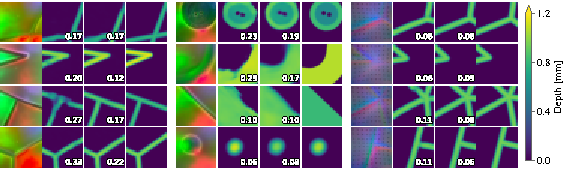
\includegraphics[width=0.97\textwidth]{figures/fig_qual.pdf}
    \caption{\textbf{Predictions on held-out frames} ($\Kreal=25$): real-only training versus MAPL on both sensors, with the per-frame contact MAE. For each object the frame shown is the one whose improvement is the object's median improvement.}
    \label{fig:qual}
\end{figure*}

\subsection{Qualitative Results}
\label{sec:qual}
Fig.~\ref{fig:qual} shows predictions at $\Kreal=25$ on held-out frames of both sensors; for every object the displayed frame is the one with the object's median improvement in contact MAE, so the examples are representative rather than selected. Real-only models blur or break thin ridges and misplace junctions; the MAPL student recovers their extent and position. On sensor B the real-only model is already close and the gain shows at junctions and at the ends of ridges.

\begin{table}[!tbp]
\centering
\tableformat
\caption{\textbf{Leave-object-out.} Errors on $1{,}244$ real frames of three objects with no real training data. Rows add simulated contacts of all 12 meshes to the real frames of the nine other objects, unless noted. The multi-sensor row is a 50-epoch run. Normal error is inside the contact region. Bold: best leakage-free.}
\label{tab:loo}
\begin{tabularx}{\columnwidth}{Xrrrrrr}
\toprule
Training data & \metrichead{Depth}{MSE} & \metrichead{Contact}{MAE} & \shortstack[c]{\strut Contact\\\strut IoU\,$\uparrow$} & \metrichead{Normal}{(deg)} & \metrichead{Rot.}{(deg)} & \metrichead{Trans.}{$L_1$} \\
\midrule
\tabloo
\bottomrule
\end{tabularx}
\end{table}

\subsection{Baseline Study: Unseen Objects}
\label{sec:loo}
Three objects are removed from all real training while their meshes remain available to simulation (Table~\ref{tab:loo}).

\noindent\textbf{Pose.} Without any data of the three objects the pose head is at chance ($64.7^\circ$). Simulated contacts of the three meshes bring it to $6.8^\circ$ with the physical renderer---calibrated from one no-contact frame and never shown a real contact---and to $5.7^\circ$ with the strict learned renderer; the leaky renderer ($4.6^\circ$) buys little, and the geometry control (same renderer, meshes removed) stays at $50.6^\circ$. Pose transfer is geometric coverage; any renderer that preserves the contact silhouette suffices. Replacing the calibrated renderer with domain-randomized sensor parameters (random LED colors and strengths, gel optics randomized per session, geometry pinned) gives $8.9^\circ$, between the calibrated ($6.8^\circ$) and single-rotation ($10.3^\circ$) rows; calibration helps by providing a consistent appearance from which the encoder extracts geometry.

\noindent\textbf{Rotation coverage.} How much of the pose space must simulation cover? Restricting simulation to one real rotation per object leaves $10.3^\circ$, two rotations $7.5^\circ$, all twelve $6.8^\circ$ (Blender rows of Table~\ref{tab:loo}); rendering the learned renderer's inputs after rotating the depth map (rotate-then-render) gives the best leakage-free pose, $4.4^\circ$. Coverage of the rotation range, not the number of synthetic frames, is the operative variable.

\noindent\textbf{Depth and normals.} Contact MAE on the unseen objects is $0.36\,$mm for real-only training, three times the seen-object value; the plain renderers reduce it by at most $4\%$ and the geometry control by almost as much ($0.340$), so this is regularization by extra frames, not object coverage. The domain-randomized Blender renderer improves contact MAE to $0.342$ and IoU to $0.601$, matching the calibrated renderer ($0.346$, $0.592$), suggesting that appearance diversity from randomized sensor parameters acts as regularization even without calibration data. A multi-sensor GAN trained on 100 simulated sensor designs does not improve over single-sensor baselines ($0.358$, $0.579$); mixing simulated sensors cannot replace real pairs. The one leakage-free renderer that helps significantly is the background-conditioned GAN-LOO: depth MSE $-13\%$, contact MAE $0.323$, IoU $0.633$, for one background frame per session; it remains far from the leaky reference ($-30\%$), which has seen real contacts of the objects. Normal error follows contact MAE. Peak-depth error is $0.05$--$0.08\,$mm for every row: the models estimate \emph{how deep} correctly and err in \emph{where} the contact lies.

\noindent\textbf{Object classification.} We add a 12-class classification head (LayerNorm + MLP on the class and mean patch tokens) and train with cross-entropy. With real data of the nine objects, the model classifies them at $94\%$ validation accuracy, but the three held-out objects score $0\%$---even when simulation provides their contact patterns through either the calibrated or learned renderer. Pose estimation transfers to unseen objects through geometry, but classification requires the appearance of the real contact, which no leakage-free renderer reproduces.

\subsection{Baseline Study: Real-Data Budget of a Renderer}
\label{sec:budget}
Table~\ref{tab:kshot} and Fig.~\ref{fig:kshot} vary the real budget of the renderers. Three regimes appear.

\noindent\textbf{Zero-shot.} Simulation alone transfers poorly for dense geometry (contact MAE $0.41\,$mm vs.\ $0.11$ with the full real set); the leaky renderer halves this but has seen $4{,}197$ real pairs.

\noindent\textbf{Few-shot ($\Kreal\le25$).} Neither leakage-free renderer improves dense error. At $\Kreal=25$ GAN-25 lowers depth MSE by $3\%$ ($0.0536\pm0.0013$ vs.\ $0.0551\pm0.0010$ over seeds) but not contact MAE or IoU; the physical renderer does the same. With $\Kreal\le25$ the real training loss reaches $10^{-4}$ within ten epochs while validation error is flat from epoch five: the model memorizes the few real frames, and synthetic frames with a different contact appearance do not regularize that memorization. Simulation does help pose at $\Kreal=10$ ($9.6^\circ\!\to\!5.2$--$5.9^\circ$), as in Sec.~\ref{sec:loo}.

\noindent\textbf{Moderate budget ($\Kreal\ge50$).} The learned renderer now helps: at $\Kreal=50$ depth MSE $0.0482\!\to\!0.0434$ ($-10\%$), contact MAE $0.283\!\to\!0.260$, IoU $0.69\!\to\!0.72$; at $\Kreal=100$ depth MSE $0.0369\!\to\!0.0311$ ($-16\%$; $0.0366\!\to\!0.0299$ over seeds, $-18\%$), contact MAE $0.235\!\to\!0.210$, IoU $0.74\!\to\!0.77$, and normal error improves in step. The physical renderer gives $-1$ to $-5\%$ MSE. The learned renderer thus needs $\approx\!50$ labeled contacts per object before its data is worth more than the frames it was trained on, and at every $\Kreal\ge50$ simulation \emph{worsens} rotation by $0.2$--$1.3^\circ$.

\subsection{Leakage, a Fidelity Proxy, and Negative Results}
\label{sec:fidelity}\label{sec:study}
\noindent\textbf{Cost of leakage.} Across Tables~\ref{tab:loo} and \ref{tab:kshot} the leaky renderer reports depth MSE reductions of $24$--$31\%$ at every budget and on unseen objects; the strict numbers are $0$--$3\%$ for $\Kreal\le25$, $10$--$16\%$ at $\Kreal\ge50$ and $5$--$13\%$ on unseen objects. The bias is largest where the pipeline is most attractive---few or no real contacts of the target---because the leaky renderer has memorized the test contacts (it reproduces validation frames with a contact-region L1 of $0.057$, half that of any strict renderer).

\begin{figure}[!tbp]
    \centering
    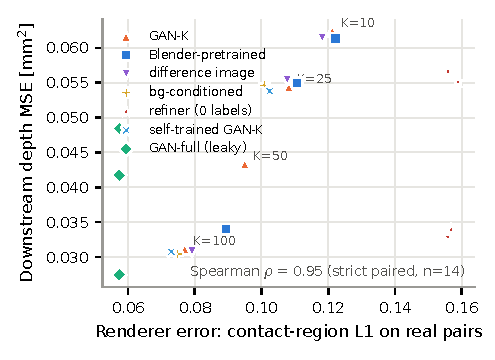
\includegraphics[width=0.85\columnwidth]{figures/fig_fidelity.pdf}
    \caption{\textbf{Renderer fidelity predicts downstream error.} Contact-region L1 between rendered and real images on held-out real (depth, image) pairs versus depth MSE of the downstream model trained with that renderer's data, for every learned-renderer variant and budget.}
    \label{fig:fidelity}
\end{figure}

\noindent\textbf{A fidelity proxy.} Rendering the depth maps of the real validation pairs and comparing with the real images gives an image error per renderer. Fig.~\ref{fig:fidelity} plots the contact-region L1 against the downstream depth MSE for every learned-renderer variant: the ordering is preserved across variants and budgets. Over the strict paired renderers, pixel metrics predict downstream error best (Spearman $|\rho|$: contact L1 $0.95$ over the 14 renderers of Fig.~\ref{fig:fidelity}, $0.97$ over the nine original ones; PSNR $0.98$, full-image L1 $0.95$), perceptual metrics worse (SSIM $0.87$, LPIPS $0.87$, contact-cropped $0.90$); adding the three leaky renderers, whose fidelity is identical while their downstream error varies with $\Kreal$, lowers every correlation to $0.75$--$0.82$, i.e.\ fidelity predicts the renderer's contribution, not the real budget. The unpaired refiner is the one exception: it is scored against the gel-warped physics render rather than its own input, so its contact L1 ($0.16$) is not comparable (Sec.~\ref{sec:unlabeled}). The proxy costs seconds and screened the variants below before downstream training.

\begin{table}[!tbp]
\centering
\tableformat
\caption{\textbf{Appearance-side and training-side variants} at $\Kreal=25$ (real validation split) and leave-object-out (unseen objects). Fidelity is the contact-region L1 of Fig.~\ref{fig:fidelity}; physics-guided variants were stopped at the fidelity stage. Only the background-conditioned renderer improves unseen-object depth.}
\label{tab:variants}
\begin{tabularx}{\columnwidth}{Xrrrrr}
\toprule
& \multicolumn{2}{c}{$\Kreal=25$} & \multicolumn{3}{c}{Unseen objects} \\
\cmidrule(lr){2-3}\cmidrule(lr){4-6}
Variant & \shortstack[c]{\strut Fidelity\\\strut $\downarrow$} & \metrichead{Contact}{MAE} & \shortstack[c]{\strut Fidelity\\\strut $\downarrow$} & \metrichead{Contact}{MAE} & \metrichead{Rot.}{(deg)} \\
\midrule
\tabvariants
\bottomrule
\end{tabularx}
\end{table}

\noindent\textbf{Which factor limits few-shot fidelity?}

Table~\ref{tab:variants} tests the hypotheses.
\emph{(i) Missing physical prior.} Pretraining the GAN on $30$k Blender pairs, conditioning it on the Blender image of the same contact, predicting a residual on top of that image, or conditioning on Blender image and background all leave contact-region fidelity unchanged or worse at $\Kreal\in\{10,25\}$ (the physical renderer's random gel-warp of $\pm3$ pixels means the conditioning image is not pixel-aligned with the target, which may limit this family).
\emph{(ii) Session illumination drift.} Session backgrounds differ by $0.05$--$0.10$ L1, more than the best renderer's total error ($0.03$); normalizing frames to a canonical background or predicting difference images improves full-image L1 by $13$--$21\%$ but leaves contact-region L1 and contact MAE unchanged (the frozen encoder is robust to the illumination field). Conditioning the renderer on the background does help on unseen objects (Sec.~\ref{sec:loo}) because it lets a renderer that never saw the object reproduce its session's illumination.
\emph{(iii) Training-side changes.} A contact-mask head with a gradient-matching loss, Blender pretraining followed by real fine-tuning, and fine-tuning with an L2-SP anchor change $\Kreal=25$ contact MAE by at most $\pm0.02\,$mm.
\emph{(iv) Domain randomization.} Randomizing the sensor's LED colors, strengths and gel optics per session while keeping the geometry stage fixed (Table~\ref{tab:variants}, ``domain rand.'') matches the calibrated renderer's contact MAE at $\Kreal=25$ ($0.320$ vs.\ $0.329$) and on unseen objects ($0.342$ vs.\ $0.346$). On sensor B at $\Kreal=25$ the match is even closer ($0.126$ vs.\ $0.125$). The calibrated renderer's advantage on pose ($6.8^\circ$ vs.\ $8.9^\circ$ on unseen objects) is consistent with a less noisy silhouette. Domain randomization is thus a viable zero-cost baseline when calibration data is not available, but it cannot close the gap to the learned renderer.
\emph{(v) Contact shading.} What remains is the appearance \emph{inside} the contact (Fig.~\ref{fig:renders}), and every result is consistent with it being the limit: strict renderers separate from real-only training only after enough contacts, leakage helps exactly because it exposes the test contacts, classification never transfers (the identity features lie entirely in the contact shading), and the residual errors are localization rather than depth-magnitude errors.

\noindent\textbf{Unpaired refiner (0 labels).} The contact-preserving refiner of Sec.~\ref{sec:refiner} translates the physical render using only unlabeled frames. On unseen objects (Table~\ref{tab:loo}) it does not improve on the calibrated render (contact MAE $0.349$ vs.\ $0.346$; on the domain-randomized render $0.353$), and its self-regularized variant is slightly worse ($0.360$): without a single labeled pair the adversarial objective is satisfied by any plausible contact shading, including a fainter one, and the ridge structure that geometry transfer needs is not what the discriminator judges. In the $\Kreal$-shot protocol, refining with the same $\Kreal=25$ frames used as unlabeled images gives the best leakage-free dense numbers at that budget (contact MAE $0.297$, IoU $0.672$, normal $27.1^\circ$; Table~\ref{tab:kshot}), a $5\%$ contact-MAE gain where no paired renderer helps, while using all of $U$ ($0.309$) or $\Kreal=100$ ($0.224$ vs.\ real-only $0.235$, GAN-100 $0.210$) adds little. The refiner's contact-region L1 ($0.156$--$0.159$, against the $\pm3\,$px-warped physics render whose identity score is $0.179$) is not comparable to the paired renderers' and is excluded from Fig.~\ref{fig:fidelity}.

\noindent\textbf{Mixing the two renderers.} Alternating physical and learned frames (Blender$\,\oplus\,$GAN) yields the average of the two on dense error and the better of the two on pose ($5.6^\circ$ on unseen objects, equal to GAN-LOO; $9.8^\circ$ across sessions, the lowest of all renderers except background normalization), so a practitioner who has both should mix them for pose and rely on the learned one for depth.
